\documentclass[conference]{IEEEtran}
\IEEEoverridecommandlockouts
% The preceding line is only needed to identify funding in the first footnote. If that is unneeded, please comment it out.
\usepackage{cite}
\usepackage{hyperref}
\usepackage{amsmath,amssymb,amsfonts}
\usepackage{algorithmic}
\usepackage{graphicx}
\usepackage{textcomp}
\usepackage{xcolor}
\def\BibTeX{{\rm B\kern-.05em{\sc i\kern-.025em b}\kern-.08em
    T\kern-.1667em\lower.7ex\hbox{E}\kern-.125emX}}
    
\graphicspath{ {./img/} }
\begin{document}

% Enriched topological learning for cluster detection and visualization
\title{Natural Language Processing for Fact-Checking and Claim Assessment\\
{\large A language model based approach}
}

\author{
\IEEEauthorblockN{Othman El houfi}
\IEEEauthorblockA{\textit{MSc Data Science \& Machine Learning} \\
CY Cergy Paris University, France \\
othmanelhoufi@gmail.com}
\and
\IEEEauthorblockN{Dimitris Kotzinos}
\IEEEauthorblockA{\textit{University Professor} \\
CY Cergy Paris University, France \\
dimitrios.kotzinos@cyu.fr}
}

\maketitle

\begin{abstract}
As false information and fake news are propagating throughout the internet and social networks, the need of fact-checking operations becomes necessary in order to maintain a truthful digital environment where general information can be reliably exploited whether in politics, finance or other domains. The need of this online claim assessment comes from the fact that fake news and false information can have a big negative impact on politics, economy (2016 USA Elections) and public health (COVID-19).\\ 
A number of solutions have been proposed to deal with this problem and limit the spread of false information, both manual and automatic. Of course the manual approaches done on websites such as \textit{PolitiFact.com}, \textit{FactCheck.org} and \textit{Snopes.com} don't construct a viable solution for the long term as the speed and scale of information propagation increase exponentially rendering this manual fact-checking operation where human fact-checkers can't scale up at the same rate limited and incapable of solving the problem.\\
Here, we present our contribution in this regard: an automated solution for fact-checking using Wikipedia as a source of truth and a state of the art language models used today for NLP tasks (BERT, RoBERTa, XLNet...) in order to classify a given claim as \textit{Supports}, \textit{Refutes} or \textit{Not enough information (NEI)}.\\
\end{abstract}

\begin{IEEEkeywords}
Natural Language Processing, Language Model, Wikipedia, Information retrieval, Text processing, Natural Language Inferencing, Fact-Checking, Document retrieval, Fake-news.
\end{IEEEkeywords}

\section{Introduction}
From a social and psychological perspective, humans have been proven irrational and vulnerable when differentiating between truth and false news (typical accuracy ranges between 55\% and 58\%) \cite{zhou2019fake}, thus fake news obtain public trust relatively easier than truthful news because individuals tend to trust fake news after repeated exposure (\textit{Validity effect}), or if it confirms their pre-existing beliefs (\textit{Confirmation bias}), or simply due to the obligation of participating socially and proving a social identity (\textit{Peer pressure}). The social sciences are still trying to comprehend the biological motivations that makes fake news more appealing to humans.\\

On the other hand, the growth of social media platforms resulted in a huge acceleration of news spreading whether true or false. As of Aug. 2017, 67\% \cite{zhou2019fake} of Americans get their news from social media. These platforms even give the user the right to share, forward, vote and participate to online discussions. All of this made the problem of fake news spreading more and more dangerous, our economies for example, are not robust to the spread of falsity, false rumors have affected stock prices and the motivations for large-scale investments, as we witnessed after a false tweet claimed that Barack Obama was injured in an explosion which caused \$130 billion drop in stock value \cite{vosoughi2018spread}. Another recent example is related to public health where rumors about COVID-19 vaccines and drug companies influenced people in their decision on getting vaccinated.\\

That being said, is there a way to monitor the spread of fake news through social media? Or more specifically, how can we differentiate between fake news and truthful news, and at what level of confidence can we do that?\\

From a computer engineering perspective, different approaches were studied:

\begin{itemize}
\item \textbf{Knowledge-based Fake News Detection \cite{chernyavskiy2021whatthewikifact}:} a method aims to assess news authenticity by comparing the knowledge extracted from to-be verified news content with known facts, also called fact-checking.
\item \textbf{Style-based Fake News Detection \cite{przybyla2020capturing}:} focuses on the style of writing, i.e. the form of text rather than its meaning.
\item \textbf{Propagation-based Fake News Detection \cite{shu2020hierarchical}:} a principled way to characterize and understand hierarchical propagation network features. We perform a statistical comparative analysis over these features, including micro-level and macro-level, of fake news and true news.
\item \textbf{Credibility-based Fake News Detection \cite{sitaula2020credibility}:} the information about authors of news articles can indicate news credibility and help detect fake news.
\end{itemize}

In this paper we will focus on a new approach that utilizes Language Models (LMs) for fact-checking. The goal is not to implement an algorithm that scans social networks for real time fake news detection, but rather we will create a model that can assess with a degree of confidence the truthfulness or falseness of a claim given by a user as an input by exploiting LMs that were already trained on Wikipedia, and fine-tune each LM for a downstream task in order to solve this classification problem.

\section{Related works}
\subsection{Language model based approach \cite{lee2020language} \cite{petroni2019language}}
A paper called \textit{"Language Models as Fact Checkers?"} done by a team from \textit{FacebookAI} and \textit{Hong Kong University of Science and Technology}, provides an example of a fact-checking model using zero-shot LM that outperforms a random baseline LM using the FEVER dataset\cite{thorne2018fever}.\\

The goal of fact-checking as mentioned previously, and relatively to this paper, is to validate the truthfulness of a given claim. Each claim is assigned to one of these labels: \textit{Supports}, \textit{Refutes} or \textit{Not enough information (NEI)} to verify.\\

This paper describes the difference between Traditional Pipeline fact-checking models and their zero-shot fact-checking LM:

\begin{itemize}
\item \textbf{Traditional pipeline:} this type of models access knowledge within an external knowledge base like Wikipedia in order to validate a claim. It involves information retrieval modules such as document retrieval and sentence retrieval.
\item \textbf{Zero-shot LM pipeline:} it replaces both the external knowledge base and the information retrieval modules with a pre-trained language model.\\
\end{itemize}

They used the publicly available 24-layer BERT-Large as our language model, which was pre-trained on Wikipedia in 2018. After fine-tuning the model they achieved 57\% in accuracy and 57\% in F1-macro score which was better than the baseline BERT model (without fine-tuning) that achieved 49\% in accuracy and 44\% in F1-macro score.

\subsection{Perplexity based approach \cite{lee2021towards} \cite{lee2020misinformation}}
In March 2021, \textit{Nayeon Lee}, \textit{Yejin Bang}, \textit{Andrea Madotto}, \textit{Madian Khabsa}, and \textit{Pascale Fung} published a paper called \textit{Towards Few-Shot Fact-Checking via Perplexity} where they propose a new approach of the powerful transfer learning ability of a language model via a perplexity score. Using a method called \textit{few-shot learning}, they built a model that outperforms major class baseline models by more than 10\% on the F1-Macro metric score.\\
In this paper the goal is to determine the veracity of a claim given some evidence, for this they define a {claim, evidence} pair. The label \emph{Supported} is assigned when relevant evidence exists that supports the claim, and \emph{Unsupported} label for the opposite case.\\
\emph{Unsupported} claims on average have higher perplexity than \emph{Supported} claims. For example, \emph{Supported} claim "Washing hands prevents the spread of diseases" has a perplexity value of 96.74, whereas the \emph{Unsupported} claim "All dogs speak English fluently" has a much higher perplexity value of 328.23.\\
The datasets used in this experiment are: Covid19-Scientific, Covid19-Social, and FEVER. As for the perplexity based experiment they used one unidirectional LM and one masked LM:
\begin{itemize}
\item $PPL_{GPT2-B}$ : a single-parameter classifier based on perplexity from GPT2-base \cite{radford2019language} (unidirectional LM)
\item $PPL_{BERT-B}$ : a single-parameter classifier based on perplexity from BERT-base \cite{devlin2018bert} (Masked LM)\\
\end{itemize}

They took into consideration the accuracy and the F1-Macro metrics for the evaluation. Because the datasets are unbalanced, they mainly consider the F1-Macro score over accuracy as an overall evaluation. The perplexity-based classifiers, especially $PPL_{GPT2-B}$, outperform all Major Class baselines across all
tasks in all settings. For instance, $PPL_{GPT2-B}$ achieved accuracy of 67.48\% and F1-macro score of 64.70\% on FEVER dataset.\\
On the other hand the classification was limited to two labels (\emph{Supported} and \emph{Unsupported}) which does not solve the entire classification problem in the FEVER dataset that provides three labels (\textit{Supports}, \textit{Refutes} or \textit{Not enough information (NEI)}).

\section{Presented method}
Most of the fact-checking algorithms today involving knowledge-based verification uses a traditional pipeline that puts in place a module for retrieving articles from an external source, another module for retrieving relevant sentences from each article, and a last module for natural language inferencing (NLI) in order to classify a claim.\\

In this paper we present a method that is fully  reliant on the powerfulness of today's best LMs. We start by fine-tuning each model for the downstream task that is claim classification using the FEVER dataset, then each model is employed to assess the validity of new input claims. This approach takes into consideration only an internal knowledge source (FEVER) for fine-tuning, that is for the learning phase, which makes the prediction phase knowledge-free rather than utilizing external knowledge sources for retrieving articles and sentences.\\

It is also important to mention that we only use LMs for classifying claims and not for generating evidence. We leave generating evidences with language models for future work.

\subsection{Dataset}
FEVER (Fact Extraction and VERification) consists of 185,445 claims generated by altering sentences extracted from Wikipedia and subsequently verified without knowledge of the sentence they were derived from. The claims are classified as Supported, Refuted or NotEnoughInfo. For the first two classes, the annotators also recorded the sentence(s) forming the necessary evidence for their judgment\cite{thorne2018fever}.

\begin{figure}[htp]
    \centering
    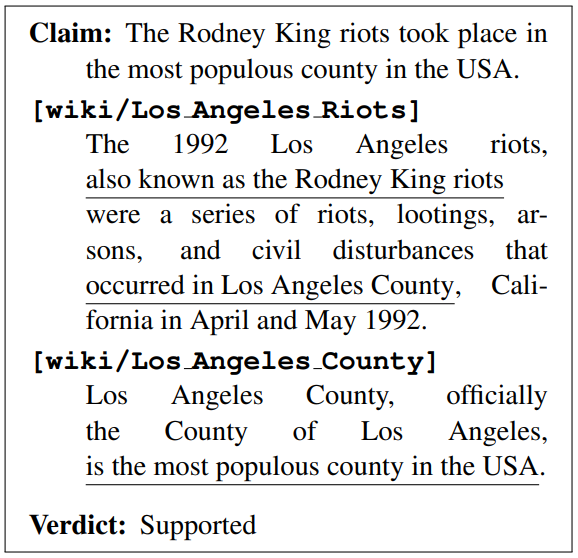
\includegraphics[scale=0.37]{fever_example.png}
    \caption{Manually verified claim requiring evidence from multiple Wikipedia pages.}
    \label{fig:fever_example}
\end{figure}


\section{Results and Analysis}
\subsection{Experimental protocol}

\subsection{Results}

\subsection{Complexity analysis}

\subsection{Conclusion of the analysis}

\section{Conclusion}

\bibliographystyle{unsrt}
\bibliography{ref}


%\begin{figure}[htp]
%    \centering
%    \includegraphics[scale=0.37]{clustering_algo.png}
%    \caption{Prototype Clustering algorithm.}
%    \label{fig:clustering_algo}
%\end{figure}

\end{document}
